\chapter{Scalable Fuzzy Ontology based Framework for Hierarchical Image Annotation}

	\label{c3}


	In this chapter, we propose a scalable ontology-based approach for automatically constructing  
	hierarchical semantic concept detectors for visual contexts, which constitutes our 
	third contribution: $C_{3}$. Having discussed fuzzy knowledge management in the previous chapter,
	we propose now to further explore such valuable knowledge in order to introduce our proposed 
	ontology driven hierarchical semantic structure in order to efficiently train and construct 
	scalable semantic concept detectors.

	The rest of this chapter is structured as follows. In Section \ref{c3_1}, we present the
	motivations of our proposal. In Section \ref{c3_2},
	we introduce our proposed scalable framework to construct semantic concept detectors. 
	Section \ref{c3_3}, introduces technical overview for an \textsc{Svm} based concept detector, then
	discusses the proposed framework scalability and efficiency through 
	the participation within the \textit{ImageClef2015}. Finally, the chapter is concluded in Section \ref{c3_4}.



	\section{Context and Motivations}
	\label{c3_1}

		As the third contribution $C_{3}$, our aim is to construct an automated 
		image annotation framework that focuses on the scalability aspect through 
		reducing semantic concept detection cost and complexity.

		Automatic photo annotation is considered as a classification problem that 
		consists in assigning a set of semantic concepts to a semantic content of
		a given image \citep{Snoek2009,Zhang2012,Piras2014}.

		Image collections are increasing staggeringly. Thus, retrieving from large-scale image 
		datasets is a challenging task \citep{Villegas2013,Villegas2014,Gilbert2015,Villegas2015}.
		The access to such considerable contents has forced the multimedia retrieval community 
		to look for advanced approaches and techniques in order to make the availability of automated 
		and efficient semantic annotation for such contents 
		\citep{Wang2011,Zhang2012,Benavent2013,Sahbi2013,Reshma2014}.

		Some previous works focused on the use of a knowledge based approach. For instance, 
		in \citep{Reshma2014} an ontology was generated and used both: (1) in training phase 
		to select images that should be used for optimizing classifiers, and (2) in testing 
		phase for deducing new annotations through concept inter-relationships.
		Seeking to contribute towards this direction, in the previous chapter, we presented a fuzzy 
		ontology based framework for enhancing a multimedia content indexing accuracy. 
		Key dimensions of this inquiry constitute the three main issues addressed by the existing 
		ontologies, namely a generic ontology structure aspect, an automated knowledge extraction 
		process for populating an ontology content, and a machine-driven context detection for 
		a multimedia content. What was accomplished in this study is a novel ontology management 
		method which is intended to a machine-driven knowledge database construction. 
		The experiment that we conducted on the \textit{ImageClef2012} dataset displayed 
		semantic improvements over a classical image annotation framework used in 
		large-scale multimedia contents.

		Our approach relies on a visual analysis of the image content. As visual features, 
		we used a \emph{k-means} \citep{Sculley2010} algorithm to classify training 
		local feature extract by \textsc{Surf} algorithm \citep{Bay2008}. For scalability, 
		our approach \revAnglais{intends} to show that we can go further in such aspect by reducing computing cost. 
		In fact, we propose an ontology based approach that alleviates the computing cost for 
		labeling a given image by candidate semantic concepts. By reading some recent papers  
		(\citep{Mller2010,Villegas2013,Villegas2014,Cappellato2015,Villegas2015} to cite a few), 
		it is obvious that there \revAnglais{is} a serious focus made on scalability through reducing
		the candidate concept list to be analyzed within an image content. Mainly, these works
		rely on dividing candidate concepts into: (1) initial concepts that can be detected directly 
		through analyzing an image content, and (2) extended concepts that can be detected through 
		reasoning with the initial ones. 

		In our second contribution $C_{2}$ (\citep{Zarka2015}), we focused on a fuzzy framework 
		for enhancing a semantic interpretation through reasoning with a given initial concept set.
		Thus, our third contribution $C_{3}$ consists in developing a fuzzy ontology to guide the
		annotation process through reducing the number of concepts to be detected.
 



	%%%%%%%%%%%%%%%%%%%%%%%%%%%%%%%%%%%%%%%%%%%%%%%%%%%%%%%%%%%%%%%%%%%%%%%%%%%%%%%%%%%%%%%%%%%%%%%%%%%%%
	\section{A Scalable Ontology driven Framework for Hierarchical Concept Detection}
	\label{c3_2}

	\subsection{Framework overview}

	In this section, we propose a scalable image annotation framework based on hierarchical annotators. 
	We investigate research works on semantic hierarchies for hierarchical image annotation.
	Our framework relies on constructing and managing a fuzzy ontology that handle a semantic 
	hierarchy. Such a hierarchy is used then to train more accurate image annotators (see figure \ref{fig1}).

	\begin{figure}[ht]
		\centering
		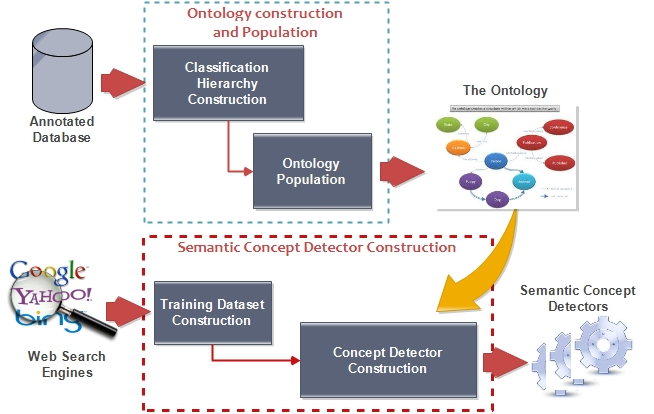
\includegraphics[scale=0.7]{graphics/contrib3:figure1}
		\caption{Ontology based semantic annotator hierarchy for image annotation}
		\label{fig1}
	\end{figure}

	Image annotation is considered as a multi-class classification problem. 
	Many approaches were proposed to handle the annotation scalability aspect 
	(large number of \revAnglais{concepts} to annotate with) through combining semantic hierarchical
	structures with classification techniques (like \textsc{Svm} : Support Vector Machine)
	\citep{Cevikalp2010,Li2010,Bannour2012,McNamara2015}.
	Mainly, two different approaches were proposed for constructing the semantic hierarchy. 
	The first one is qualified as top-down method: the semantic hierarchy is \revAnglais{built} through
	recursive class set clustering \citep{Cevikalp2010}. The second one is qualified as
	bottom-up method: the hierarchy is  defined by agglomerative partitioning of the classes
	\citep{Li2010}. Furthermore, two different approaches were proposed also for hierarchical
	image classification: the first is the \textit{Binary Hierarchical Decision Trees} 
	(\textsc{Bhdts})\citep{Cevikalp2010}, and the second is the \textit{Decision Directed 
	Acyclic Graphs} (\textsc{Ddags}) \citep{Gao2011}.

	Let $C = \{c_{1} , c_{2}  , \dots , c_{N}\}$ be a set of $N$ semantic concept. 
	The \textsc{Ddags} approach trains $N * (N-1)/2$ binary classifiers and uses a 
	\textsc{DAG} to decide if an image $image$ belongs or not to a semantic concept 
	class $c_{i} \in C$. At each given node at a distance $d$ from the tree root, $d$
	semantic concept classes are eliminated, and $N-d$ decision nodes remain to be evaluated. 
	The \textsc{Bhdts} approach \revAnglais{handles} the semantic hierarchy as a binary tree: concept 
	classes are clustered hierarchically into two subsets. This clustering step is iterated 
	until a single concept class set is reached. For every clustering step,  an \textsc{Svm} 
	classifier is trained in order to decide if an image $image$ could be annotated by the first or 
	the opposite semantic concept class. A total of $log_{2}(N)$ \textsc{Svm} classifiers are 
	trained and used for analyzing a test image.  Despite the fact that these two approaches enable 
	accurate classifiers, they handle semantic hierarchy as binary structures which requests 
	a considerable structure to handle with large amount of concept classes.

	Considering that \textsc{Bhdt} approach aims to optimize the \textsc{SVM} classifiers 
	accuracy through reducing the unnecessary comparisons \citep{Cevikalp2010}, 
	we are motivated to use such an \revAnglais{approach} in our scalable image annotation framework.

	In our proposed framework, we aim to define a new method for constructing a hierarchical 
	classifiers for scalable image annotation. At first, an annotated image dataset is analyzed to 
	construct the hierarchy tree for concept classes. Then, and for every level of the defined 
	tree structure, an \textsc{Svm} is trained for predicting if a test image $image$ belongs 
	to the first concept class set or the second one. By starting by the first level  (root node), 
	the hierarchy is walked until reaching leafs nodes through computing classifier votes  (see figure \ref{fig3_2}).

	\begin{figure}[ht!]
		\centering
		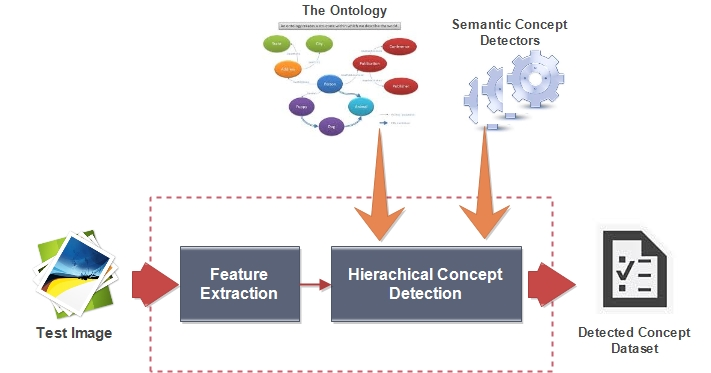
\includegraphics[scale=0.7]{graphics/contrib3:figure2}
		\caption{Ontology based Hierarchical image classification}
		\label{fig3_2}
	\end{figure}

	Our method is inspired from fuzzy decision tree based method \citep{Wang2015,Bujnowski2015} 
	to extract uncertain knowledge in a classification problem. Fuzzy set theory is used to model
	the tree structure. Thus, our proposed approach is based on a fuzzy ontology that handles such 
	a decision tree. In what follows, we discuss the structure of our fuzzy ontology, we show how 
	we populate its content, and how to infer available knowledge in order to use the hierarchical 
	classifiers to annotate a test image accurately.

	\subsection{Ontology Structure}
		The ontology structure is based on three conceptual \revAnglais{classes:} the semantic 
		concept $\mathsf{Concept}$, the hierarchical node $\mathsf{Node}$, and the test image $\mathsf{Image}$.
		We define also a set of relationships between these conceptual classes (see table \ref{tab1}).
		\begin{table}[ht!]
			\centering
			\caption{Semantic Relationships between conceptual classes}
			\begin{tabular}{ c c p{5cm}  }
			\hline
			\textbf{\small Relationships} 	& \textbf{\small Definition}	&\textbf{\small Meaning} \\
			\hline \hline
			
			$\mathsf{isIndexedBy}$	& 
			$(\langle{}\mathsf{Image},\mathsf{Concept}\rangle:\mathsf{isIndexedBy}) \geq p_{1}$ 
			& The image $\mathsf{Image}$ is annotated by the concept $\mathsf{Concept}$ by a fuzzy weight $p_{1}$  \\
			\hline
			
			$\mathsf{votesFor}$		& 
			$(\langle{}\mathsf{Node},\mathsf{Image}\rangle:\mathsf{votesFor}) \geq p_{2}$ 
			& The \textsc{Svm} for the node $\mathsf{Node}$ votes for the image $\mathsf{image}$ by a fuzzy weight $p_{2}$  \\
			\hline
	
			$\mathsf{existsIn}$		& 
			$(\langle{}\mathsf{Concept},\mathsf{Node}\rangle:\mathsf{existsIn}) \geq p_{3}$ 
			& The image $\mathsf{image}$ exists in the node $\mathsf{Node}$ by a fuzzy weight $p_{3}$  \\
			\hline
	
			$\mathsf{isChildOf}$	& 
			$(\langle{}\mathsf{Node},\mathsf{Node}\rangle:\mathsf{isChildOf})$ 
			& The first node $\mathsf{Node}$ has a semantic concept subset of the second node 
			$\mathsf{Node}$ \\
			\hline
		\end{tabular}
		\label{tab1}
	\end{table}


The relationship $\mathsf{isChildOf}$ depicts that a node $node_{1} \in \mathsf{Node}$ is a child of another node $node_{2} \in \mathsf{Node}$. This relationship is used then for modeling the semantic hierarchy for concept classes.

The relationship $\mathsf{existsIn}$ enumerates for each node $node \in \mathsf{Node}$ the contained set of concept classes. A concept $concept \in \mathsf{Concept}$ can \revAnglais{exist} in many nodes, but for separate levels.
 
The relationship $\mathsf{votesFor}$ is used when an image $image$ is being annotated and the hierarchy is walked from the root node to the leafs. A node $node \in \mathsf{Node}$ votes for an image $image \in \mathsf{Image}$ by a fuzzy weight $p_{2}$ when a \textsc{Svm} classification on that image predicts that the image $image$ could \revAnglais{be }annotated by the set of semantic concepts that exists in the node $node$.
	
Finally, the relationship $\mathsf{isIndexedBy}$ depicts that an image $image \in \mathsf{Image}$ is annotated by the concept $concept \in \mathsf{Concept}$ by a fuzzy weight equal to $p_{1}$.
		
The proposed ontology structure is used to enable handling the hierarchical classifiers, to trace the hierarchy walk for classifying a given test image, and then to model the set of semantic concepts that annotate that image (see figure \ref{fig3}). In what follows, we expose the population process for our ontology, then, we discuss the reasoning process used to guide and assist the hierarchical annotation.


\begin{figure}[ht!]
	\centering
	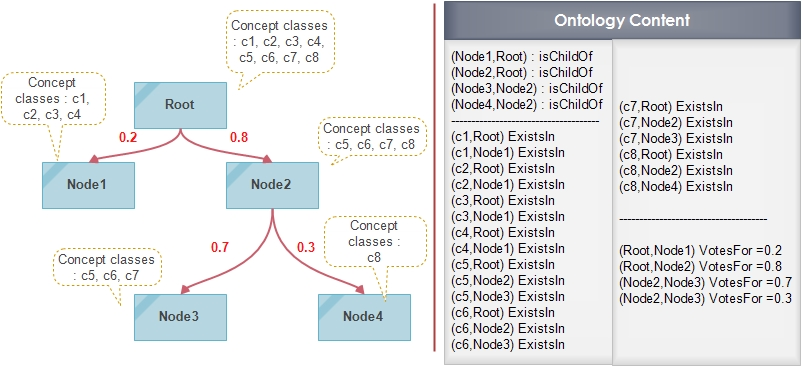
\includegraphics[scale=0.72]{graphics/contrib3:structure}
	\caption{Ontological Hierarchy content for image annotation}
	\label{fig3}
\end{figure}
		\subsection{Ontology population}
		
Given a defined set of semantic concepts, we start by clustering it through analyzing annotated image dataset provided by the \textit{ImageCLEF 2015 Scalable Concept Image Annotation} task.  

At first, we apply a binary clustering for the whole concept set, and we define two new nodes in the ontology $node_{1}$ and $node_{2}$.
We use a \textit{k-means} clustering algorithm with $k=2$.
 Then, each concept is instantiated within the ontology, and for every concept $concept$ that belongs to the node $node$, a new relationship $\mathsf{existsIn}$ is instantiated between $concept$ and $node$. This process is recursively called on $node_{1}$ and $node_{2}$ until a sub-node contains only one semantic concept class, or the clustering process seems unable to cluster a given semantic concept classes. At each iteration, the new defined nodes are populated within the ontology through instantiating the $\mathsf{isChildOf}$ relationships. 

		\subsection{Hierarchical classificators construction}

Once the hierarchical structure is defined through the above mentioned recursive binary clustering, an \textsc{Svm} based classifier is trained for all the nodes that belong to the same level. As training images, we select some development images for every concept that belongs to a node. In section \ref{label1}, we detail the development image dataset used for the training task.

\begin{figure}[ht!]
	\centering
	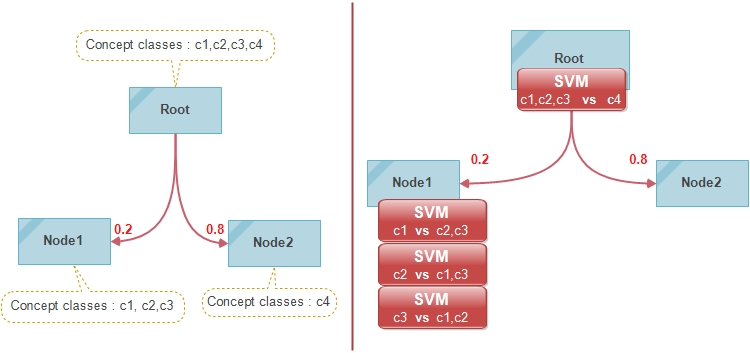
\includegraphics[scale=0.8]{graphics/contrib3:figure3}
	\caption{Hierarchical SVM classificator construction}
	\label{fig4}
\end{figure}

At a given level, two possible nodes are figuring (see figure \ref{fig4}). By exploring $\mathsf{existsIn}$ relationships, we construct a training image dataset. For the first node (see node \emph{Root} in figure \ref{fig4}), and for each concept that belongs to that node, a subset of images that are annotated by this concept are selected to be training images for corresponding node.

For a leaf node (see node \emph{Node1} in figure \ref{fig4}), we proceed as follow: let $C_{m} = \{ c_{1}, c_{2}, \dots, c_{k}\}$ be a set of $k$ concepts that belongs to the node $node_{m}$. We construct then $k$ classifiers. Each classifier is related to a given concept and trained against the other concepts. Then, and for a classifier $f$ of a concept $c_{f} \in C_{m}$, we train an \textsc{Svm} classifier based on two image sets: the first set is based on images that are annotated by the concept $c_{f}$, and the other set is based on images that are annotated by the other concepts ($C_{m} \setminus c_{f}$).

For a leaf node that \revAnglais{contains} only one concept class (see node \emph{Node2} in figure \ref{fig4}), no \textsc{Svm} classifier will be constructed. And an image annotation for this concept will be computed through the leaf node classification vote.

		\subsection{Reasoning}

We start reasoning from the root node (top node) of the constructed fuzzy tree (see figure \ref{fig3}). For a given node, we compute the values of the membership functions ($\mu$) for the child nodes through firing the corresponding \textsc{Svm} classifiers. The classification results (the vote) are populated into the fuzzy ontology through instantiating the $\mathsf{votesFor}$ relationship.

%Cheng2010
%Chen2009
In order to improve reasoning accuracy and to minimize the decision tree walk (which will also minimize the number of \textsc{Svm} classifiers to be fired), we define a \textit{Fuzziness control threshold} $\theta_{r} = 0.1$: given two sub-nodes $node_{1}$ 
and $node_{2}$, firing the \textsc{Svm} classifier at this level provides two membership function values $\mu_{1}$ for $node_{1}$ and  $\mu_{2}$ for $node_{2}$. Then, we compute $\theta_{r} = | \mu_{1} - \mu_{2} |$.

if $\theta_{r} \leq 0.1$, then we could not be sure if the \textsc{Svm} classifier is discriminative to judge if the content of a test image belongs to the first or to the second node. We proceed so to walk both sub-nodes ($node_{1}$ and $node_{2}$). For the opposite case ($\theta_{r} > 0.1$), the reasoner walks only the node that has the greater membership function value ($\mu$). 

Given the example in figure \ref{fig3}, the \textsc{Svm} classifier of the node $root$ computed $\mu_{1} = 0.2$ for the node $Node1$, and 
$\mu_{2} = 0.8$ for the node $Node2$. Then, the reasoning algorithm stops walking the node $Node1$ and proceeds to walk the $Node2$ since
$\theta_{r} = 0.8-0.2 = 0.6$ and $0.1 \leq 0.6$.

A leaf node can contain a set of concept classes, or only one concept class. In the first case, and for every contained concept class, an \textsc{Svm} classifier is fired for that concept against the other contained concept classes. The classification result is populated in the ontology through the instantiation of the relationship $\mathsf{isIndexedBy}$ between the concept class and the test image. The fuzzy weight for the new relationship is computed as an average of $\mu$ values computed from the root node to the leaf one. 
 In case of a single concept class, a new $\mathsf{isIndexedBy}$ relationship is instantiated within the ontology between that concept and the test image. The fuzzy weight \revAnglais{is computed} as in the first case.

Our proposed fuzzy decision tree reasoner assists the annotation of a given test image through firing recursive trained \textsc{Svm} classifiers in order to optimize the number of concept to be detected. Such an optimization should reduce also the computing cost of a given test image annotation process.

In the next section, we expose how we construct an \textsc{Svm} classifier for each node in the constructed fuzzy hierarchical semantic structure of concept classes.


	%%%%%%%%%%%%%%%%%%%%%%%%%%%%%%%%%%%%%%%%%%%%%%%%%%%%%%%%%%%%%%%%%%%%%%%%%%%%%%%%%%%%%%%%%%%%%%%%%%%%%
	\section{Experiments and Results}
	\label{c3_3}
		
		In this section, we discuss the obtained experimental results from our participation in the 
		\textit{Imageclef 2015} (within the \textit{Scalable Concept Image Annotation} task).
		In such an experiment, we look particularly in the assessment of our approach scalability, 
		rather than the semantic enhancement.
		
		In the rest of this section, we start by presenting the used dataset and metrics for 
		the evaluation, we, then, show how we build hierarchical concept detectors in accordance 
		with what was presented in the previous section. And finally, we discuss the obtained results.

		\subsection{Datasets Description}
			The image dataset provided by the \textit{ImageClef 2015} evaluation campaign is 
			constructed through querying popular search engines (mainly \textsc{Google}, \textsc{Bing} 
			and \textsc{Yahoo!}). A total of $500~000$ images \revAnglais{were} gathered \citep{Gilbert2015}.

			The test dataset contains all the defined $500~000$ images. And the development dataset 
			contains $5~520$ annotated images taken from the test dataset. A total of $251$ semantic
			concepts where used to annotated the content of the development set of images.

			For each image in the dataset, a full text description of the image content is 
			provided through extracting text content from the web-page where the image is located.

		\subsection{Evaluation metrics}
			In \textit{imageclef 2015} \textit{Scalable Concept Image Annotation} task, the annotation 
			accuracy is evaluated using the \textsc{Map} metric.
			
			Another metric is used: the \textsc{Pascal Voc} \citep{Everingham2015}. But the 
			latter evaluates not only the annotation accuracy, but also the semantic 
			concept localization. Since our approach \revAnglais{desn't} handle yet such \revAnglais{an} ability, 
			we consider only the \textsc{Map} metric.


		%%%%%%%%%%%%%%%%%%%%%%%%%%%%%%%%%%%%%%%%%%%%%%%%%%%%%%%%%%%%%%%%%%%%%%%%%%%%%%%%%%%%%%%%%%%%%%%%%%%%%
		\subsection{\textsc{Svm} Classifier Construction}
			In our participation within \textit{ImageCLEF 2015 Scalable Concept Image Annotation} task,
			we aimed basically to evaluate the scalability aspect of our preliminary automatic annotation 
			framework. For semantic concept detector/annotator, we have not really defined an original approach, 
			but we implemented state-of-the-art bags of quantized local features and linear 
			classifiers learned by support vector machines. In fact, and as pointed in \cite{Piras2014}, 
			bag-of-features and codebook approach has 
			gained a great attention by image classification and annotation community 
			as it showed notable semantic accuracy 
			\citep{Jurie2005,Gemert2008,Mylonas2009,Ngo2010,Grana2013,Hidaka2013,Kanehira2014,Xu2014,Elleuch2015}.
			%\cite{Mylonas2009,Kanehira2014,Elleuch2015}.
			In what follow, we expose how we construct \textsc{Svm} classifiers for semantic concept detection and annotation.

			\subsubsection{Construct a learning dataset}
				\label{label1}
				Image annotation has always been heavily dependent \revAnglais{on} good development datasets. 
				First, datasets were mainly hand-collected. However, and recently, several researches 
				attempt to automate such a laborious task. Re-ranking images gathered from popular 
				Image search engines (\textsc{Google}, \textsc{Yahoo!}, \textsc{Bing}, \dots) 
				can construct automatically an image learning dataset \citep{Fergus2004,Fergus2005,Schroff2011}.

				As a development dataset, we have not used one provided by the \textit{ImageCLEF
				2015 Scalable Concept Image Annotation task}. In fact, not all the concepts were annotated. 
				We relied then on \textsc{Flickr} image search engine to obtain image set and construct 
				a learning dataset. We used so the information provided with concept list to 
				query the search engine and we gathered first 100 result images for each given concept.

				At the outset, it seems to be curious to use an external data source as a development dataset. 
				Our aim is to explore available on-line data-sources (like search engines) to train non 
				annotated semantic concepts.


			\subsubsection{Local Feature Extraction}
				Our framework extracts \revAnglais{feature} from an input image through a robust local feature extractor.
				We followed a basic and state-of-the-art framework for such purpose (as described in \citep{Piras2014}).
				Leading extractors for such a purpose \revAnglais{include} \textit{Scale Invariant Feature 
				Transform} (\textsc{Sift}) and \textit{Speeded Up Robust Features} (\textsc{Surf}).
				Local feature descriptors handle a pixel within an image by analyzing 
				its neighborhood pixels. Many different descriptors and interest-point
				detectors were proposed and discussed in the literature. While the \textsc{Sift} 
				descriptor \citep{Lowe2004} is considered as the most widely used descriptor, 
				\textsc{Surf}  \citep{Bay2008} is known as robust local feature extraction
				to various image perturbations.

				Our framework extracts local features and descriptors using \textsc{Surf}. Such a choice is
				argued by \textsc{Surf} concise descriptor length (64 floating point values).
				The \textsc{Surf} implementation that we used is provided by 
				\textsc{OpenCv} \citep{Bradski2008}.

				For query image analysis, local features are extracted and mapped into 
				nearest computed cluster centroids. The query image is then handled by a 
				vector that represents defined visual bag-of-words.

			\subsubsection{Classification of local Features and Constructing the bag-of-words model}
				After extracting local features, a bag-of-words model is used to represent these descriptors. 
				The \revAnglais{latters} are extracted from training images and are grouped into $N$ clusters of 
				visual words using \textit{k-means}.	
				Each  defined descriptor is classified into its cluster centroid by computing the 
				\textit{Euclidean distance} metric. For our runs, we choose a value of $N = 100$. 
				This value is argued by a balance between high bias (under-fitting) and high variance (over-fitting).
				
				In order to alleviate the computing cost of \textit{k-means} clustering, we used 
				\textit{Mini Batch k-means} 
				\cite{Sculley2010} as an alternative to the \textit{k-means} algorithm for clustering massive 
				datasets. \textit{Mini Batch k-means} reduces the computational cost by handling fixed size 
				subsample instead of all the data in the database. This strategy reduces the amount 
				of distance to be computed at each clustering iteration.

			\subsubsection{Learning Algorithm}
				The learning algorithm consists in training one-vs.-one linear \textsc{Svm}
				to operate in the bag of \textsc{Surf} feature space. Training images are classified
				through a histogram vector conctructed in the \textit{k-means} based clustering.
				We used a linear kernel for our \textsc{Svm} based learning algorithm in view of its simplicity and 					computational efficiency in training and classification: $K(x,y) = x^{T}y+c$.

				Basically, \textsc{Svm} are binary classifier. For a given detector, an image 
				is annotated by one of two distinct groups. A one-vs.-one scheme is used in which 
				each \textsc{Svm} trained for each combination of individual classes. 
				The \textsc{Svm} implementation used in our runs is given by \textsc{Scikit-Learn} 
				library \citep{Pedregosa2011}.

			\subsubsection{Decision}

				As an \textsc{Svm} decision function, a class membership probability estimation 
				fits the decision values.
		
				\textsc{Scikit-Learn} library uses a \textsc{Platt Scaling} in order to 
				calibrate the \textsc{Svm} classifier to produce, in addition to class 
				predictions, probabilities. When the \textsc{Svm} is trained, an optimization 
				process is called to optimize parameter vectors $A$ and $B$ such \revAnglais{that:}
				$P(y|X) = 1/ (1+exp(A*f(X) + B))$ where $f(X)$ 
				is the signed distance of a sample  from the hyperplane.

			

		\subsection{Experiments with \textit{ImageClef 2015}}

			Our goal behind our participation in \textit{ImageClef 2012} is to assess the proposed 
			ontology based hierarchical concept detection scalability. However, and unlike the 
			scalability assessment presented in the previous chapter (where we tested the 
			scalability of the system to handle a large-scale image dataset), we aim to test if 
			our approach could be scalable when the number of semantic concepts \revAnglais{increases}. Our idea 
			behind the ontology based hierarchical concept detection consists in filtering the 
			concepts to be detected: not all the concept detectors will be called in the detection process.



			\subsubsection{Image Semantic Annotation Evaluation}
			For the image annotation, we only annotated only $300~000$ images of 
			the $500~000$ images provided in the test dataset. Furthermore, we used just 
			low resolution images (thunbnail)
			instead of the full resolution images. In fact, the large amount \revAnglais{of} images to 
			be annotated has forced us to reduce the quality of processed images in the 
			aim to accelerate the annotation computational cost. Yet, we haven't \revAnglais{proceeded
			to annotate} the full image dataset (only $300.000$ images).

			The tables \ref{tabres1} and \ref{tabres2} display the obtained results in terms of
			semantic annotation accuracy. We think that a full size image dataset annotation with
			more tweaked \textsc{Svm} classifiers should give better results. 
			Furthermore, fuzzy ontology based semantic enhancement (described in the previous 
			chapter \citep{Zarka2015}) should also enhance our framework annotation accuracy.

			\begin{table}[ht]
				\centering
				\caption{\textsc{ImageClef 2015}: $MAP\_0\_Overlap$ Runs evaluation}
				\begin{tabular}{ l| l l }
				\hline
				\textbf{\small } 	& \textbf{\small MAP} &	 \\
				\hline \hline
		
				\textbf{\small Best run}  & {\small $0,795403$}	& {\small(/SMIVA/21.run)} \\
				\textbf{\small Worst run} & {\small$0,0305398$}	& 
					{} \\
				\textbf{\small Average}	  & {\small$0,31046$} 	&  \\
				\textbf{\small Our best run~~}& {\small$0,0366072$} 	&  {\small(position $85/89$)} \\
				\hline
				\end{tabular}
				
				\label{tabres1}
			\end{table}

			\begin{table}[ht]
				\centering
				\caption{\textsc{ImageClef 2015}: $MAP\_0.5\_Overlap$ Runs evaluation}
				\begin{tabular}{ l| l l }
				\hline
				\textbf{\small } 	& \textbf{\small MAP} &	 \\
				\hline \hline
				\textbf{\small Best run}  & {\small $0,659507$}		& {\small(/SMIVA/21.run)} \\
				\textbf{\small Worst run} & {\small $0,000231898$}	& {\small(} \\
				\textbf{\small Average}	  & {\small $0,18673$} 		&  \\
				\textbf{\small Our best run~~}& {\small$0,0161687$} 	&  {\small(position $75/89$)} \\
				\hline
				\end{tabular}
				
				\label{tabres2}
			\end{table}

			As illustrated in tables \ref{tabres1} and \ref{tabres2}, the system \textsc{Smiva} 
			\citep{Pravin2015} showed great annotation performance. This system annotates images
			not only in the basis of its visual content, but also through analyzing textual information 
			in the web page where the analyzed image is localized. For our evaluation, we only used visual analysis.


			
			\subsubsection{Scalability Evaluation}

			We would remind that our objective is to alleviate the computation cost of the 
			image annotation through a proposed framework that is based on an ontology 
			reasoning driven hierarchical concept detector.

			For the training process, we trained the \textsc{Svm} classifiers in about $100$ hours
			(we used 100 learning images per a concept). This task was executed on 
			a \revAnglais{modern} machine (Intel $i5$ processor with $16$ GB RAM memory).
	
			The annotation task was done on $10$ machines (each one has one core 
			CPU and $1$ GB of RAM). The annotation of $300~000$ images elapsed about $1~633$ hours 
			(without taking into consideration the \textsc{Vps} parallel computing).

			Our framework annotates a test image with an average of $19.615$ seconds (the maximum record 
			was $597.250$ seconds and the minimum one was $0.066$ second). 
			And for a given test image, an average of $52$ \textsc{Svm} classifiers were fired
			(the maximum was $175$ and the minimum was $6$). Our framework has reduced 
			the number of \textsc{Svm} classifiers to be fired in order to annotate a given test image.

			We can conclude that our proposed framework reduced the number of requested semantic 
			concept detector to annotate an image: from $251$ concept detectors, to an average of $52$
			ones. Then, the time required to annotate an image is decreased by $80\%$





	%%%%%%%%%%%%%%%%%%%%%%%%%%%%%%%%%%%%%%%%%%%%%%%%%%%%%%%%%%%%%%%%%%%%%%%%%%%%%%%%%%%%%%%%%%%%%%%%%%%%%
	\section{Conclusion}
	\label{c3_4}

	In this chapter note, we described our annotation framework for scalable ontology driven 
	semantic image annotation. We discussed our ontology based framework for reducing the number of 
	concepts to be detected for a given image. We developed a state-of-the art bag-of-words based 
	concept detector (that uses \textsc{Surf} feature extractor and \textit{k-means} classification).
	Then, concept detectors are selected through reasoning with a fuzzy ontology content. Thus, not all 
	the concept detectors are used for a given image. 

% 	In our experiment, we showed how the use of such a method could reduce the number of concept 
% 	detectors to be used in order to efficiently annotate a large-scale image dataset. While the 
% 	obtained results were not really impressive, we still believe 
% 	that our framework can reveal better results through tweaking local feature extraction and
% 	training, and exploiting semantic enhancement through fuzzy reasoning. 
% 	Thus, we are considering potential future directions to further improve our proposed framework. 
	
	The main discussed contribution was to propose a scalable framework for
		multimedia content analysis. We focused then on the use of an ontology in order to construct 
		fast semantic concept detectors. Although the promising obtained results, we believe that the
		implementation of these constructed detectors within \emph{Hadoop/MapReduce} and even \emph{GPU} 
		based runtime-environment (like \textsc{Cuda, OpenCL} \citep{Mahmoudi2015,Osipyan2015,Dantas2015,Peters2015}
		could enable more efficiency for multimedia content analysis.


